\documentclass{article}
\usepackage{a4wide}

\usepackage{amsmath}
\usepackage{amssymb}
%\usepackage[notref,notcite]{showkeys}
\usepackage[utf8]{inputenc}
\usepackage{latexsym}
\usepackage{graphicx}
\usepackage{subcaption}
\usepackage{pgf,tikz}
\usetikzlibrary{backgrounds}
\usepackage{bbold}
\usepackage{animate,media9}
\usetikzlibrary{arrows}
\usepackage[linkbordercolor=white]{hyperref}
\hypersetup{pdfborder=0 0 0}
\usepackage{float}
\usepackage{color}
\usepackage{enumitem}
\usepackage[normalem]{ulem}
\usepackage[title]{appendix}
\usepackage{lipsum}

\newcommand\blfootnote[1]{%
  \begingroup
  \renewcommand\thefootnote{}\footnote{#1}%
  \addtocounter{footnote}{-1}%
  \endgroup
}

\topmargin -1cm
\textheight21cm
\textwidth15cm 
\oddsidemargin1cm

\newtheorem{theorem}{Theorem}[section]
\newtheorem{lemma}{Lemma}[section]
\newtheorem{corollary}{Corollary}[section]
\newtheorem{prop}{Proposition}[section]
\newtheorem{definition}{Definition}[section]
\newtheorem{remark}{Remark}
\newtheorem{example}{Example}
\newtheorem{notation}{Notation}

\definecolor{ddgreen}{rgb}{0,0.4,0.4}
\definecolor{dgreen}{rgb}{0,0.65,0}


\newenvironment{proof}{\noindent{\textsc{Proof.}}}
{$\hfill\Box$\vspace{0.1 cm}\\}
\newenvironment{proofof}[1]{\noindent{\textsc{Proof of #1.}}}
{$\hfill\Box$\vspace{0.1 cm}\\}


\newcommand{\R}{\mathbb R}

\newcommand{\N}{{\mathbb N}}

\newcommand{\F}{{\mathcal F}}
\newcommand{\NF}{{\mathcal NF}}

\newcommand{\BV}{BV}
\newcommand{\tv}{\mathrm{TV}}
\newcommand{\tvp}{\mathrm{TV}^+}
\newcommand{\PV}{\mathrm{PV}}
\renewcommand{\L}[1]{\mathbf{L^{\pmb{#1}}}}
\newcommand{\Ll}[1]{\mathbf{L_{loc}^{\pmb{#1}}}}
\newcommand{\C}[1]{{\mathbf C^{\pmb{#1}}}}
\newcommand{\Cc}[1]{{\mathbf {C_c^{\pmb{#1}}}}}
\newcommand{\W}[1]{{\mathbf W^{\pmb{#1}}}}
\newcommand{\Wl}[1]{{\mathbf{W_{loc}^{\pmb{#1}}}}}


\newcommand{\eps}{\varepsilon}
\newcommand{\lam}{\lambda}
\newcommand{\A}{{\cal A}}
\newcommand{\ruf}[1]{(\ref{#1})}
\newcommand{\norm}[1]{\left\| #1 \right\|}
\newcommand{\abs}[1]{\left\vert #1 \right\vert}
\newcommand{\RP}{Riemann Problem }
\newcommand{\wc}{\rightharpoonup}
\newcommand{\KK}{\mathcal{K}}
\newcommand{\Rf}{\mathcal{RS}^f}
\newcommand{\Rr}{\mathcal{RS}}
\newcommand{\Rsol}{\mathcal{RS}}
\newcommand{\s}{\subseteq}
\newcommand{\jumps}{\mathcal{J}}
\newcommand{\shocks}{\mathcal{S}}
\newcommand{\raref}{\mathcal{R}}
\newcommand{\pt}{\partial_t}
\newcommand{\px}{\partial_x}
\newcommand{\tr}[3]{\mathcal T^{#1}_{#2}\left( #3 \right)}
\newcommand{\fhi}{\varphi}
\newcommand{\Rsl}{\Rsol_{1,2}}
\newcommand{\Rsp}{\Rsol_{2,1}}
\newcommand{\sx}[1]{\rho_l^{#1}}
\newcommand{\dx}[1]{\left(\rho_r^{#1}, q_r^{#1} \right)}
\newcommand{\dom}{\Omega_f \cup \Omega_c}

\newcommand{\fhil}{\fhi(\rho^l, q^l)}
\newcommand{\fhim}{\fhi(\rho^m, q^m)}
\newcommand{\fhir}{\fhi(\rho^r, q^r)}

\newcommand{\rhol}{(\rho^l, q^l)}
\newcommand{\rhom}{(\rho^m, q^m)}
\newcommand{\rhor}{(\rho^r, q^r)}

\DeclareMathOperator{\argmin}{argmin}
\DeclareMathOperator{\sgn}{sgn}
\DeclareMathOperator{\diver}{div}
%\DeclareMathOperator{\tv}{\hbox{Tot.Var.}}
\definecolor{aliceblue}{rgb}{0.94, 0.97, 1.0}




\title{Inverse design for the one-dimensional Burgers equation}



\author{
Thibault Liard% \footnote{DeustoTech, University of Deusto, 48007 Bilbao, Basque Country, Spain (\texttt{thibault.liard@deusto.es}).} \footnote{Facultad de Ingenieria, Universidad de Deusto, Avda.Universidades, 24, 48007, Bilbao - Basque Country-Spain.}
 \footnote{Chair of Computational Mathematics, Fundaci\'on Deusto Av. de las Universidades 24, 48007 Bilbao, Basque Country, Spain.}
\and
Enrique Zuazua\footnotemark[\value{footnote}] \footnote{Chair in Applied Analysis, Alexander von Humboldt-Professorship, Department of Mathematics Friedrich-Alexander-Universitat, Erlangen-Nurnberg, 91058 Erlangen, Germany.} \footnote{Departamento de Matem\'aticas, Universidad Aut\'onoma de Madrid, 28049 Madrid, Spain.}%\footnote{DeustoTech, University of Deusto, 48007 Bilbao, Basque Country, Spain (\texttt{enrique.zuazua@deusto.es}).} \footnote{Facultad de Ingenieria, Universidad de Deusto, Avda.Universidades, 24, 48007, Bilbao - Basque Country-Spain}
}


\date{}
\begin{document}
\maketitle





\section{The problem}

We consider the following one-dimensional Burgers equation 
\begin{equation} \label{eq} \left\{ \begin{array}{l}
\partial_t u(t,x)+\partial_x f(u(t,x))=0, \quad (t,x)\in \R^+ \times \R, \\
u(0,x)=u_0(x),
\end{array}\right.
\end{equation}
where $u$ is the state, $u_0$ is the initial state and  the flux function $f$ is defined by $f(u)=\frac{u^2}{2}$. Kruzkov's theory \cite{Kru70} provides existence and uniqueness of a  solution  of \eqref{eq} with initial datum $u_0 \in L^{\infty}(\mathbb R)$. This solution is called a weak-entropy solution, denoted by $(t,x) \to S_t^+(u_0)(x)$. For a given function $u^T$, we introduce the backward entropy  solution $(t,x) \to S^-_{t}(u^T)(x)$  as follows: 
for every $t\in [0,T]$, for a.e $x\in \mathbb R$,  
$$S^-_{t}(u^T)(x)= S^+_{t}(x\to u^T(-x))(-x).$$
We study the problem of inverse design for \eqref{eq}. This problem consists in  identifying the set of initial data evolving to a given target at a final time.  \ \\
 \ \\
Due to the time-irreversibility of the Burgers equation, some target functions are unattainable from weak-entropy solutions of this equation, making the inverse problem under consideration ill-posed. To get around this issue, we introduce the following  optimal control problem 

\begin{equation} \tag{$\mathcal{O}_T$}\label{opt2} \inf_{u_0\in \mathcal{U}^0_{\text{ad}}} J_0(u_0):=\Vert u^T(\cdot)-S_T^+(u_0)(\cdot)\Vert_{L^2(\mathbb R)},\end{equation}

where $u^T$ is a given target function and the class of admissible initial data $\mathcal{U}^0_{\text{ad}}$ in \eqref{opt2} is defined by 
\begin{equation} \label{admissible_set}\mathcal{U}^0_{\text{ad}}=\{u_0\in BV(\mathbb R) \slash \Vert u_0 \Vert_{BV( \mathbb R)} < C \,  \text{and } \text{supp}(u_0)\subset K_0\}.\end{equation}
Above, BV stands for functions of bounded variation and  $C>0$ is a constant large enough. The study of \eqref{opt2} is motivated by the minimization of the sonic boom effects generated by supersonic aircrafts \cite{Cle95,AC12,APZ16b}.  \ \\

\par To solve the optimal control problem \eqref{opt2}, some difficulties arise from a  theoretical  and  numerical point of view. 
\begin{itemize}
\item Since the  entropy solution $u$ of \eqref{eq} may contain shocks even if the initial datum is a smooth function, this generates important added difficulties that have been the object of intensive study in the past, see  \cite{BM95,BM95b,BJ98,BJ99} and the references therein. In particular, the authors make sense of the derivative of $J_0$ in \eqref{opt2} in a weak way by requiring  strong conditions on the set of initial data. This leads to require that entropy solutions of \eqref{eq} have a finite number of non-interacting jumps.
\item When $J_0$ is weakly differentiable,  gradient descent  methods have been implemented in \cite{CPZ08,CPZ10,APZ16a} to solve numerically the optimal problem \eqref{opt2}. In the cases where it was applied successfully, only one possible initial datum emerges, namely the backward entropy solution $S_T^-(u^T)$.This is mainly due to the numerical viscosity that numerical schemes introduce to gain stability. To find some multiple minimizers, the authors in  \cite{GZ17}  use a filtering step in the backward adjoint solution.   
\end{itemize}

Dans \cite{LZ19}, we fully characterize the set of minimizers of the optimal control problem \eqref{opt2}.

\begin{theorem}  \label{main:optimal} Let $u^T\in BV(\mathbb R)$. The optimal control problem \eqref{opt2}  admits multiple optimal solutions. Moreover, for a.e $T>0$, the initial datum $u_0\in BV(\mathbb R)$ is an optimal solution of \eqref{opt2} if and only if $u_0 \in BV(\mathbb R)$ verifies $S_T^+(u_0)=S_T^+ (S_T^-(u^T))$.
\end{theorem} 
A characterisation of the set $\{u_0 \in BV(\mathbb R), S_T^+(u_0)=S_T^+ (S_T^-(u^T))\}$ is given in \cite{CP19}. An illustration of Theorem \ref{main:optimal} is given in Figure \ref{projection}. 
\begin{figure}[h!]
  \centering
      \includegraphics[width=0.65\linewidth]{projection2.pdf}
  \caption{The backward-forward  solution $S_T^+(S_T^-(u^T))$ is the projection of $u^T$ onto the set of attainable target functions. The shaded area in red at time $t=0$ represents the set of minimizers of \eqref{opt2}  \label{projection}.}
\end{figure}  \ \\
The proof of Theorem \ref{main:optimal} is structured as follows. From  \cite[Theorem 3.1, Corollary 3.2]{CP19}, \cite[Corollary 1]{GZ17} or \cite{GG14}, there exists $u_0\in BV(\mathbb R)$ such that $S^+_T(u_0)=q$ if and only if $q$ satisfies  the one-sided Lipschitz condition \cite{BC98,Gla08,Ole57,Daf10}, i.e 
$ \partial_x q \leq \frac{1}{T}  \text{ in } \mathcal{D}'(\R).$
 Thus, the optimal problem \eqref{opt2} can be rewritten as  follows. 
 \begin{equation} \label{opt5} \min_{q\in \mathcal{U}^T_{\text{ad}}} J_1(q):=\Vert u^T-q \Vert_{L^2(\R)}, \end{equation}
where the admissible set $\mathcal{U}^T_{\text{ad}}$ is defined by 
$$\mathcal{U}^T_{\text{ad}}=\{ q\in BV(\mathbb R) \slash \, \, \partial_x q \leq \frac{1}{T} \,  \, \text{and } \Vert q \Vert_{BV( \mathbb R)} \leq C \, \text{and }\text{Supp}(q)\subset K_1 \}.$$
Above, $K_1$ an open bounded interval large enough.  Note that the optimal problem \eqref{opt5} is not related to the PDE model \eqref{eq}. We prove that $q=S_T^+ (S_T^-(u^T))$ is a critical point of \eqref{opt5} using the first-order optimality conditions applied to \eqref{opt5} and the full characterization of the set $ \{u_0 \in BV(\mathbb R) \slash S_T^-(u_0)=S_T^-(u^T)\}$ given in \cite[Theorem A.2]{LZ19}. \ \\




\section{Numerical simulations} %From Theorem \ref{main:optimal}, we start by constructing an approximate solution of  the backward-forward solution $S_T^+(S_T^-(u^T))$


In \cite[Section 3]{LZ19}, we  implement a wave-front tracking algorithm to construct numerically the set of  minimizers of \eqref{opt2}.  We consider for instance, a target function $u^T$  defined by 
\begin{equation} \label{uT} u^T(x)=\left\{\begin{array}{ll}
2 &\text{if} \, \,x\in (-0.2,1.1)\bigcup(2,3.1)\bigcup (4.1,5.3)\bigcup (6.1,7.2), \\
-1 & \text{otherwise}.
\end{array}\right.
\end{equation}
From Theorem \ref{main:optimal},  the backward solution $S_T^-(u^T)$ is an  optimal solution of \eqref{opt2} and  $u_0$ is an optimal solution of \eqref{opt2} if and only if  $S_T^+(u_0)=S_T^+ (S_T^-(u^T))$. In Figure \ref{uTplotting}, the target function $u^T$, the backward solution $S_T^-(u^T)$ and  the backward-forward solution $S_T^+ (S_T^-(u^T))$ are plotted.  \ \\
\begin{figure}[H]
\begin{center}
\scalebox{1}{
\begin{tikzpicture}[node distance=1cm, auto,]
 



\node[inner sep=0pt] (russell) at (0,-1.2)
   {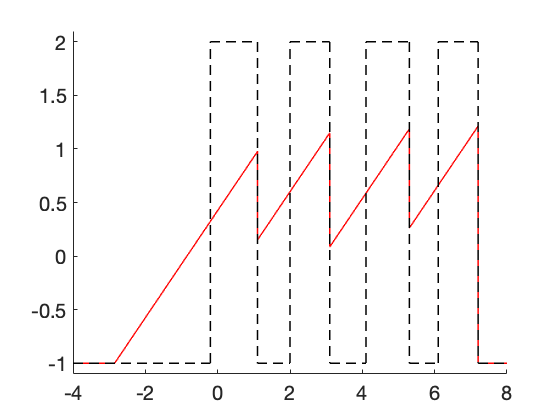
\includegraphics[width=0.5\textwidth]{ex_final.png}};
   \node[inner sep=0pt,] (russell) at (-4,5)
   {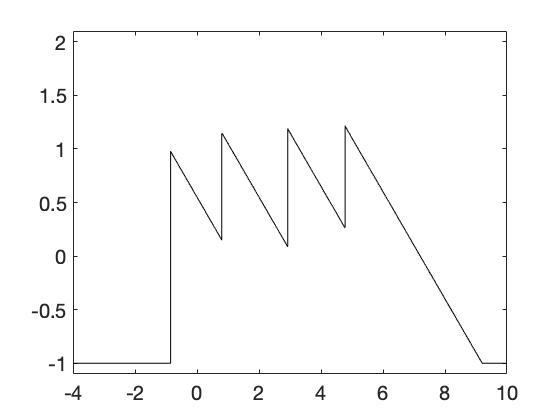
\includegraphics[width=0.5\textwidth]{ex_Stmoins.png}};
     \node[inner sep=0pt,] (russell) at (4,5)
   {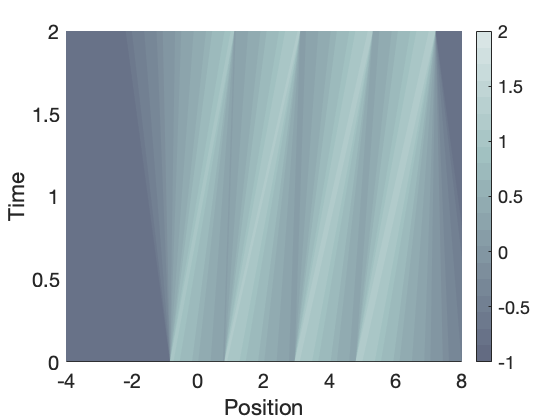
\includegraphics[width=0.5\textwidth]{WFTforward.png}};
%  \node[inner sep=0pt,] (russell) at (-4,0)
 %  {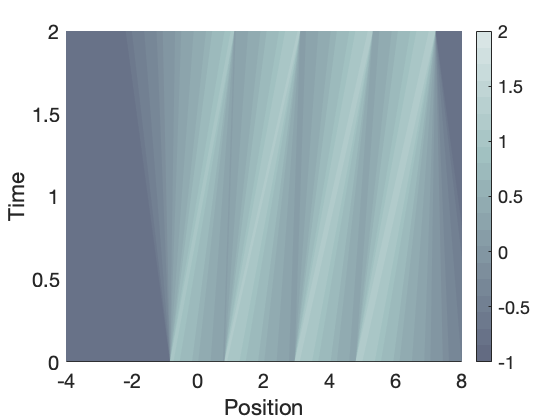
\includegraphics[width=0.5\textwidth]{WFTforward.png}};
   
   
 %   \node[inner sep=0pt,] (russell) at (-4,0)
 %  {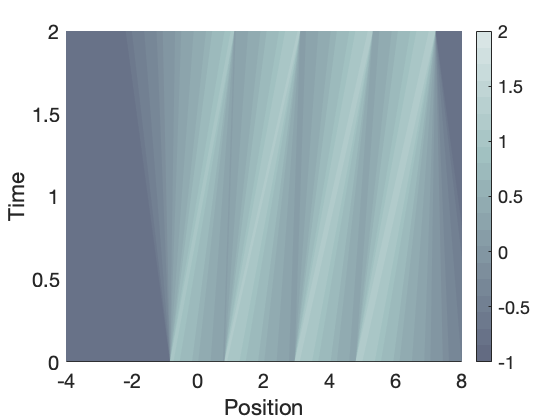
\includegraphics[width=0.4\textwidth]{WFTforward.png}};
   %  \node[inner sep=0pt,] (russell) at (0,0)
  % {\includegraphics[width=0.4\textwidth]{exM5.png}};
 % \node[inner sep=0pt,] (russell) at (4,0)
 %  {\includegraphics[width=0.4\textwidth]{exM6.png}};
   
  \node[rectangle,
           rounded corners,
           draw=white, very thin,
           text width=15em,
           minimum height=2em,
           text centered]  at (0,-4.2){$u^T$  and $\textcolor{red}{x\to S^{+}_T(S^{-}_T(u^T))(x)}$};   
           
             \node[rectangle,
           rounded corners,
           draw=white, very thin,
           text width=20em,
           minimum height=2em,
           text centered]  at (-4,1.8){$x\to S^{-}_T(u^T)(x)$};  
           
              \node[rectangle,
           rounded corners,
           draw=white, very thin,
           text width=20em,
           minimum height=2em,
           text centered]  at (4,1.8){$(t,x)\to S^{+}_t(S^{-}_T(u^T))(x)$};   
              
\end{tikzpicture}
}

\end{center}
\caption{Plotting of the target function $u^T$ defined in \eqref{uT}, the optimal solution $S_T^-(u^T)$ and the backward-forward solution $\textcolor{red}{S^{+}_T(S^{-}_T(u^T))}$  \label{uTplotting}}
\end{figure}

\par Note that $S_T^+(S_T^-(u^T))$ has four different shocks located at $x=1.1$, $x=3.1$, $x=5.3$ and $x=7.2$. If we use a conservative numerical method as Godunov scheme,  the approximate solution of $S_T^+(S_T^-(u^T))$ doesn't have shocks because of numerical viscosity that numerical schemes introduced, see Figure  \ref{God}. This implies that only one minimizer of \eqref{opt2} can be constructed using a Godunov scheme, which is the backward entropy solution $S_T^-(u^T)$. When a wave-front tracking algorithm is implemented, the approximate solution of $S_T^+(S_T^-(u^T))$ has shocks since we track the discontinuities from $u^T$ to  $S_T^+(S_T^-(u^T))$. This implies that all initial data $u_0$ that coincide with the approximate solution of $S_T^+ (S_T^-(u^T))$ can be recovered, see \cite[Section 3]{LZ19}.  \ \\
\begin{figure}[H]
\begin{center}
\scalebox{0.80}{
\begin{tikzpicture}[node distance=1cm, auto,]



   \node[inner sep=0pt,] (russell) at (-4,-2)
 {\animategraphics[controls,loop,width=0.6\textwidth]{12}{animation_God_WFT}{}{}};
  \node[inner sep=0pt,] (russell) at (5,-2)
{\animategraphics[controls,loop,width=0.6\textwidth]{8}{animation_God_WFT_zoom}{}{}};





           


\end{tikzpicture}
}

\end{center}
\caption{Approximation solution of $S_T^+(u_0)$ with $u_0$ an $N$-wave constructed with  \textcolor{red}{a wave-front tracking algorithm (in red)} and \textcolor{blue}{a Godunov scheme (in blue)} \label{God}}
\end{figure}


 
  
   
  \par  At the  left top of Figure \ref{video}, the weak-entropy solution of \eqref{eq}  with initial data $S_T^-(u^T)$ coincides with $S_T^+ (S_T^-(u^T))$ at time $T$. In Figure \ref{video}, three other optimal solutions of \eqref{opt2} $u_0$ are plotted. In particular, we have $S_T^+ (u_0)=S_T^+ (S_T^-(u^T))$. 





\begin{figure}[H]
\begin{center}
\scalebox{1}{
\begin{tikzpicture}[node distance=1cm, auto,]
 

\node[inner sep=0pt,] (russell) at (-4,2)  {\animategraphics[controls,loop,width=0.5\textwidth]{12}{animation_0}{}{}};

\node[inner sep=0pt,] (russell) at (4,2)  {\animategraphics[controls,loop,width=0.5\textwidth]{12}{animation_1}{}{}};

\node[inner sep=0pt,] (russell) at (-4,-5)  {\animategraphics[controls,loop,width=0.5\textwidth]{12}{animation_3}{}{}};

\node[inner sep=0pt,] (russell) at (4,-5)  {\animategraphics[controls,loop,width=0.5\textwidth]{12}{animation_4}{}{}};

           
              
   
   
  

\end{tikzpicture}
}
\end{center}
\caption{ Plotting of four optimal solutions of \eqref{opt2}.  The weak-entropy solutions of \eqref{eq} associated to the four optimal solutions $\textcolor{blue}{u_0}$ evolve to the backward-forward solution $S_T^+(S_T^-(u^T))$ at time $T=2$, i.e
$S_T^+(\textcolor{blue}{u_0})=\textcolor{red}{S_T^+(S_T^-(u^T))}$ \label{video}}
\end{figure}











\footnotesize
\bibliographystyle{plain}
\bibliography{biblio}
\end{document} 



